\documentclass[a4paper,12pt,fleqn]{extreport} %размер бумаги устанавливаем А4, шрифт 14пунктов
\usepackage[T1,T2A]{fontenc}
\usepackage[utf8]{inputenc}%включаем свою кодировку: koi8-r или utf8 в UNIX, cp1251 в Windows
\usepackage[english,russian]{babel} %используем русский и английский языки с переносами
\usepackage{amssymb,amsfonts,amsmath,mathtext,cite,enumerate,float} %подключаем нужные пакеты расширений
\usepackage{graphicx} %хотим вставлять в диплом рисунки?
\graphicspath{{"C:/Users/Salmon/Dropbox/SaintGobain/Report2/pictures/"}} %путь к рисункам
\usepackage{amsfonts}
%\usepackage{indentfirst} % включить отступ у первого абзаца
\long\def\comment{}


\usepackage{calc}
\usepackage{epstopdf}
\usepackage{setspace}

\usepackage{fancyvrb}
\DefineShortVerb{\|}

\begin{document}

\section{Вычисление поля для однородного потока}

Решаем уравнение:

\begin{equation}
\begin{aligned}
\tilde{\varphi}(x_2, y_2, k_z, \omega) = \frac{\exp (-i k_z z_1)}{4 \pi^2} G(x_2 - x_1, y_2 - y_1) + \\
+ \iint_{\Omega} \left[\frac{\omega^2}{c^2} - (\frac{\omega}{c} - M(x,y) k_z)^2\right] \tilde{\varphi}(x,y,k_z,\omega) G(x_2 - x, y_2 - y) dx dy,
\end{aligned}
\end{equation}

где $\Omega$ - область, в которой поток имеет ненулевую скорость (вне $\Omega$ ядро уравнения нулевое), $x_2$ и $y_2$ - координаты микрофона, $x_1$ и $y_1$ - координаты источника.

Решаем итерационным способом:

\begin{equation}
\begin{aligned}
\tilde{\varphi_0}(x_2,y_2) = \frac{\exp (-i k_z z_1)}{4 \pi^2} G(x_2 - x_1, y_2 - y_1)\\
\tilde{\varphi_n}(x_2, y_2, k_z, \omega) = \frac{\exp (-i k_z z_1)}{4 \pi^2} G(x_2 - x_1, y_2 - y_1) + \\
+ \iint_{\Omega} \left[\frac{\omega^2}{c^2} - (\frac{\omega}{c} - M(x,y) k_z)^2\right] \tilde{\varphi_{n-1}}(x,y,k_z,\omega) G(x_2 - x, y_2 - y) dx dy,
\end{aligned}
\end{equation}

\subsection{Код}

Расстоние от источника к приемнику, расстояния от каждой точки области $\Omega$ до приемника:

\begin{verbatim}
|r2_min_r1 = sqrt((x_source-x_micro)^2 + (y_source-y_micro)^2) ; |
|r_min_r2  = sqrt((X-x_micro ).^2 + (Y-y_micro ).^2) ;|
\end{verbatim}
Для каждого $k_z$ и каждой частоты.

Задал функцию Грина, доопределил в нуле, чтобы не было особенности:
\begin{verbatim}
|wave = -1i/4 * besselh(0, 1, k_xy *r_array) ;|
|r_array = [0, r_array] ;|
|wave = [0, wave] ;|
\end{verbatim}
Функция Грина в области $\Omega$:
\begin{verbatim}
|G_xy_mat = interp1(r_array, wave, dist) ; |
\end{verbatim}
Функция Грина от источника до приемника:
\begin{verbatim}
|G_r2r1 = interp1(r_array, wave, r2_min_r1) ;|
\end{verbatim}
Функция Грина от каждой точки области $\Omega$ до приемника:
\begin{verbatim}
|G_r2r = interp1(r_array, wave, r_min_r2) ;|
\end{verbatim}
Задал ядро интегрального уравнения $K$,

\begin{equation}
K(x,x_2,y,y_2) = \left[\frac{\omega^2}{c^2} - \left(\frac{\omega}{c} - M(x,y)k_z\right)^2\right] G(x_2-x, y_2-y) dx dy
\end{equation}
\begin{verbatim}
|kernel = (- M.^2 * k_z^2 + 2 * M * k * k_z) * step^2 ; |
|K = G_r2r .* kernel  ;|
\end{verbatim}
Задал начальное приближение для итерационной процедуры,
\begin{verbatim}
|f_x = exp(-1i *k_z *(z_micro - z_source)) * G_r2r1 ; |
|y_nmin1 = f_x * ones(sz,1) ;|
|y_n = y_nmin1 * 0 ;|
\end{verbatim}
Делаю, пока относительная невязка следующего приближения с предыдущим не станет маленькой
\begin{verbatim}
|while (abs(nev) > 1e-2)|
\end{verbatim}
Считаю следующее приближение. Сделал $K$ матрицей, умножил его на предыдущее приближение:
\begin{verbatim}
|y_n = f_x + K * ones(1, sz) * y_nmin1 ;|
\end{verbatim}
Посчитал невязку, в какой-то понятной мне форме:
\begin{verbatim}
|nev = sum(sqrt(y_nmin1.^2 - y_n.^2)) / sum(sqrt(y_nmin1.^2 + y_n.^2)) ;|
\end{verbatim}
В следующий раз буду в интеграл подставлять функцию от $x$ и $y$:
\begin{verbatim}
|y_nmin1 = y_n ;|
\end{verbatim}
Из функции от $x$ и $y$ суммированием хочу получить функцию от $x_2, y_2$. Мне казалось, это аналогично интегрированию по $x,y$:
\begin{verbatim}
|y_n_num = sum(y_n) ;|
\end{verbatim}

\section{Для неоднородного потока}
\subsection{Уравнение}

Конвективное волновое уравнение:
\begin{equation}
\frac{\partial^2 p}{\partial t^2} + 2U \nabla\left(\frac{\partial p}{\partial t}\right) + \left(U_z^2 - c^2\right) \nabla^2 p = 0,
\end{equation}

Сделаем Фурье по времени, разделим на $c^2$, припишем правую часть:
\begin{equation}
-\frac{\omega^2}{c^2}p - \frac{2iM\omega}{c}p + (M^2 - 1) \nabla^2 p = \frac{1}{8 \pi^3 c^2} \delta(x-x_1) \delta(y-y_1) \delta(z-z_1)
\end{equation}

Влево перенесем однородное уравнение Гельмгольца, а вправо - все остальное:

\begin{equation}
\Delta p + \frac{\omega^2}{c^2}p = M^2 \Delta p - \frac{2iM\omega}{c}\nabla p - \frac{1}{8 \pi^3 c^2} \delta(x-x_1) \delta(y-y_1) \delta(z-z_1)
\end{equation}

Функция Грина в $3D$:

\begin{equation}
G(\vec{r}) = \frac{1}{4 \pi} \frac{e^{ik\|\vec{r}\|}}{\|\vec{r}\|}.
\end{equation}

Запишем уравнение Липмана-Швингера для этого волнового уравнения:

\begin{equation}
\begin{aligned}
\Delta p = \frac{e^{ik\|\vec{r} - \vec{r_1}\|}}{32 \pi^4 c^2\|\vec{r} - \vec{r_1}\|} + \iint_\Omega \left[M^2 \Delta - \frac{2iM\omega}{c}\nabla\right]p(x,y,z,\omega) \frac{1}{4\pi} \frac{e^{ik\|\vec{r}_2 - \vec{r}\|}}{\|\vec{r}_2 - \vec{r}\|} d\vec{r}
\end{aligned}
\end{equation}

\subsection{Струя}

\begin{figure}[h]
	\center{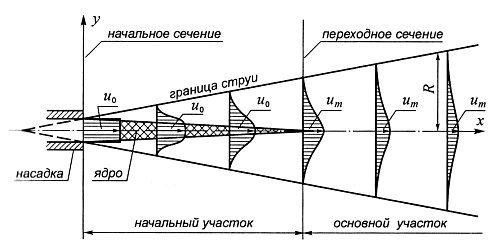
\includegraphics[width=0.8\linewidth]{struya}}
	\caption{Струя}
	\label{ris:image}
\end{figure}


Есть исходник $Mach.m$, он делает трехмерную картинку потока. Функция зависит от сеток $x,y,z$, скорости потока $U$, диаметра сопла $d$. Строится профиль скорости на основе модели, взятой из литературы по авиации. Наука мутная, все формулы в ней эмпирические.

Выбирается параметр турбулентности $a$, для не очень турбулентого потока (у нас такой) он равен $a = 0.066-0.08$. Раствор потока увеличивается линейно, угол раствора равен $\beta$, $\tan \beta = 3.4 a$. Радиус струи $r_{s} = x \tan\beta$, где $x$ - ось, совпадающая с осью потока.

Делится на два участка: начальный и основной. Начальный участок - участок после сопла, на котором у струи еще есть ламинарное ядро. На основном участке ламинарное ядро уже схлопнулось. Диаметр ядра равен диаметру сопла на начальном сечении и спадает до нуля на переходном сечении. Полюс струи - точка, где пересекутся границы струи, если продолжить их за плоскость сопла. Полюс струи находится с другой стороны от сопла, чем струя.

Расстояние от полюса струи до переходного участка:

\begin{equation}
x_{tr} = 0.96*r_0/a,
\end{equation}
где $r_0$ - радиус сопла, а $a$ - показатель турбулентности.

От полюса струи до начального участка:

\begin{equation}
x_0 = 0.29 r_0/a
\end{equation}

Считается, что на начальном участке струи амплитуда на оси струи держится постоянной, а на основном спадает как

\begin{equation}
\frac{U}{U_0} = 0.96 \frac{r_0}{ax}
\end{equation}

Если считать от начального сечения, будет:
\begin{equation}
\frac{U}{U_0} = \frac{0.48 d_0}{a + 0.145 d_0/l} l,
\end{equation}
где $l$ - это расстояние от начального сечения. Это называется формула Абрамовича.

\subsection{Код для решения уравнения}

Сетку задал трехмерную, $(x,y,z)$ на трехмерной сетке задал операции производной $\nabla = \frac{\partial}{\partial x} + \frac{\partial}{\partial y} + \frac{\partial}{\partial z}$ и второй производной $\Delta = \frac{\partial^2}{\partial x^2} + \frac{\partial^2}{\partial y^2} + \frac{\partial^2}{\partial z^2}$. Матрицы проверял, ошибок не увидел.

Вычисляю матрицу для числа Маха в каждой точке. Поскольку надо будет потом умножить эту матрицу так, чтобы она давала веса в производных, делаю ее размерности $N \times N$, где $N$ - количество точек.
\begin{verbatim}
    Mxy = Mach(X, Y, Z, V, d, dz) ;
    Mxy_mat = repmat(Mxy.', cub, 1) ;
\end{verbatim}

То, что дальше, делаю для каждой частоты. Вычислил матрицу, которая стоит в качестве ядра в уравнении Липпмана-Швингера. Также вычисляю начальное приближение в качестве свободного члена в уравнении. $p_ip1$ - это следующий шаг в приближении, тут он просто инициализуется.	
	
\begin{verbatim}
    Matr = -2i*Mxy_mat*omega.*D_3d/c0 + Mxy_mat.^2.*D2_3d ;
    p_i = 1/32/pi^4*exp(1i*k*r1_min_r)./r1_min_r./(Mxy.^2 - 1) ;
    p_ip1 = X ;
\end{verbatim}

Сделал конечное количество итераций, чтобы просто понять, работает или нет. 

\begin{verbatim}
for i=1:8
		if (i>1) p_i = p_ip1 ; end ;
	    p_ip1 = 1/(4*pi)*sum(Matr * (p_i .* exp(1i*k*r2_min_r)./r2_min_r)...
	    *dx *dy *dz ) ;       
end
\end{verbatim}

Ответ получается гигантский. Что делать - непонятно.

\end{document}
